\documentclass[12pt]{article}
\usepackage{cite}
\usepackage{amsmath}
\usepackage[a4paper, margin=0.8in, bottom=1.0in]{geometry}
\usepackage{graphicx}
\graphicspath{ {images/} }
\usepackage{listings}
\usepackage{textcomp}
\usepackage[utf8]{inputenc}
\usepackage[english]{babel}
\usepackage{color}

\definecolor{dkgreen}{rgb}{0,0.6,0}
\definecolor{gray}{rgb}{0.5,0.5,0.5}
\definecolor{mauve}{rgb}{0.58,0,0.82}

\lstset{frame=tb,
  language=Python,
  aboveskip=3mm,
  belowskip=3mm,
  showstringspaces=false,
  columns=flexible,
  keywordstyle=\color{blue},
  commentstyle=\color{dkgreen},
  basicstyle={\small\ttfamily},
  numbers=none,
  breaklines=true,
  breakatwhitespace=true,
  tabsize=3
}

\title{Cryptanalysis of Book-Caesar-RSA Cipher}

\author{Samanvitha Basole and Shubham Pachpute\\
\\
CS 265 Cryptography and Computer Security\\
\\
San Jose State University
}

\date{\today}

\begin{document}
\maketitle

% ~~~~~~~~~~~~~~~~~~~~~~~~ PROBLEM STATEMENT ~~~~~~~~~~~~~~~~~~~~~~~~
\section{Problem Statement}
...


% ~~~~~~~~~~~~~~~~~~~~~~~~ APPROACH ~~~~~~~~~~~~~~~~~~~~~~~~
\section{Approach}
In this paper, we solve the BCR cipher consisting of a three-stage cascade: Altered book, Caesar, and RSA. Each stage uses the output of the previous one as input as shown in Figure \ref{fig:arch}.
\begin{figure}[h]
  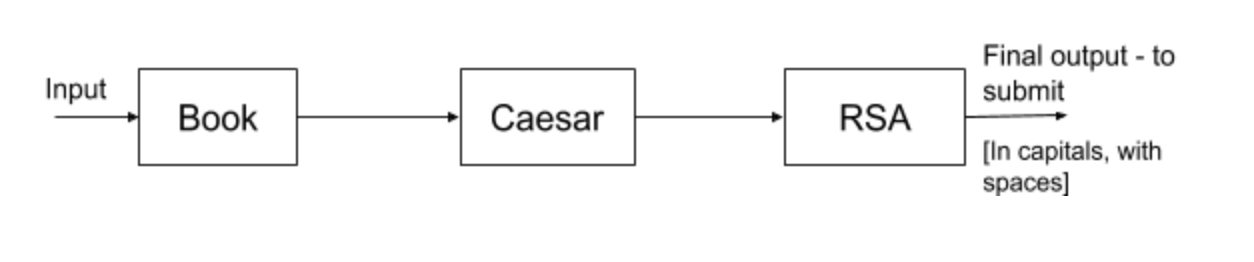
\includegraphics[scale=0.8]{3_stage}
  \caption{General Architecture}
  \label{fig:arch}
\end{figure}
We discuss the high-level algorithm design of Book, Caesar, and RSA ciphers, then we present the algorithm pseudocode and part of the implementation. Next, we explain our decryption process and analysis achieved through computational experiments. Finally, we provide screenshots of our solution and submission.


% ~~~~~~~~~~~~~~~~~~~~~~~~ ALGORITHM DISCUSSION ~~~~~~~~~~~~~~~~~~~~~~~~
\section{Algorithms Discussion}
\subsection{Book Cipher}
\subsection{Caesar Cipher}
Caesar cipher is a simple substitution cipher in which the alphabet is shifted a certain number of characters based on the key. It is a symmetric key algorithm, that is, the same key is used for encryption and decryption \cite{busta2002encryption}. \\
We show the following example to demonstrate encryption and decryption using Caesar cipher: 
Given a Caesar cipher with a left shift of 3, we first convert letters to numbers:
\begin{lstlisting}
Letters: 	A   B   C   D   E   F   ...   X    Y    Z
Numbers: 	0   1   2   3   4   5   ...   23   24   25
\end{lstlisting}
To encrypt the plaintext 'ATTACK AT DAWN', we
\begin{itemize}
\item Transfom each letter in the plaintext into a number using the above scheme
\item Apply the rule: (number + key) mod 26 to each transformed number
\item Tranform each number back to its corresponding letter using the same scheme above
\end{itemize}
The result is the following ciphertext XQQXZH XQ AXTK. \\ 
Decryption is done in a similar way except the following rule is applied in the second step: (number - key) mod 26.

\subsection{RSA}

% ~~~~~~~~~~~~~~~~~~~~~~~~ ALGORITHM PSEUDOCODE ~~~~~~~~~~~~~~~~~~~~~~~~
\section{Algorithms Design}
\subsection{Book}
\subsection{Caesar}
The hex input consists of letters and numbers while the key consists of numbers as offset. The below code demonstrates the main logic of the algorithm:
\begin{lstlisting}
output_str = ""
for eachChar in hex_string:
    try:
    	# if eachChar is a number
        digit = int(eachChar)
        output_str += str((digit - int(YY)) % 10)
    except:
    	# if eachChar is a letter
        output_str += letters[(letters.index(eachChar) + int(XX)) % 26]
\end{lstlisting}
\subsection{RSA}

% ~~~~~~~~~~~~~~~~~~~~~~~~ DECRYPTION ~~~~~~~~~~~~~~~~~~~~~~~~
\section{Decryption and Analysis}
...

% ~~~~~~~~~~~~~~~~~~~~~~~~ SUBMITTING SOLUTION ~~~~~~~~~~~~~~~~~~~~~~~~
\section{Solution Submission}
...

\bibliography{references}
\bibliographystyle{plain}

\end{document}